\chapter{Cristaux I~: le cristal parfait et les métaux}\label{ch:b1:crystals-metals}

Un fil de cuivre peut être étiré plus fin qu'un cheveu sans se rompre~;
un morceau de sel vole en éclats sous le marteau. Un forgeron chauffe une
barre de fer jusqu'à ce qu'elle rougeoie, la martèle, la plonge dans
l'eau, et la barre en ressort bien plus dure qu'elle n'y est entrée. La
différence entre ces comportements tient à la façon dont les atomes
sont empilés dans le solide. La plupart des solides sont des \omterm{def:b1:crystals-metals:crystal}{cristaux}~:
leurs atomes occupent un \omterm{def:b1:crystals-metals:lattice}{motif} qui se répète, identique, des milliards
de fois dans toutes les directions. Ce chapitre décrit ces \omterm{def:b1:crystals-metals:lattice}{motifs},
dénombre leurs atomes, mesure leur \omterm{def:b1:crystals-metals:compactness}{compacité} et repère les espaces
vides entre eux, puis s'en sert pour comprendre les métaux et les
alliages. Le chapitre suivant applique les mêmes outils aux solides
ioniques, covalents et moléculaires.

\begin{recall}
Les métaux perdent facilement leurs \omterm{def:b1:quantum-numbers:configuration}{électrons de valence}~: leurs
énergies d'ionisation et leurs \omterm{def:b1:periodicity:electronegativity}{électronégativités} sont faibles
(\cref{ch:b1:periodicity}). Les rayons atomiques ont été définis à la
\cref{def:b1:periodicity:radius}. La masse volumique, propriété étudiée
en physique, est supposée connue~: $\rho = m/V$.
\end{recall}

\begin{omfigure}
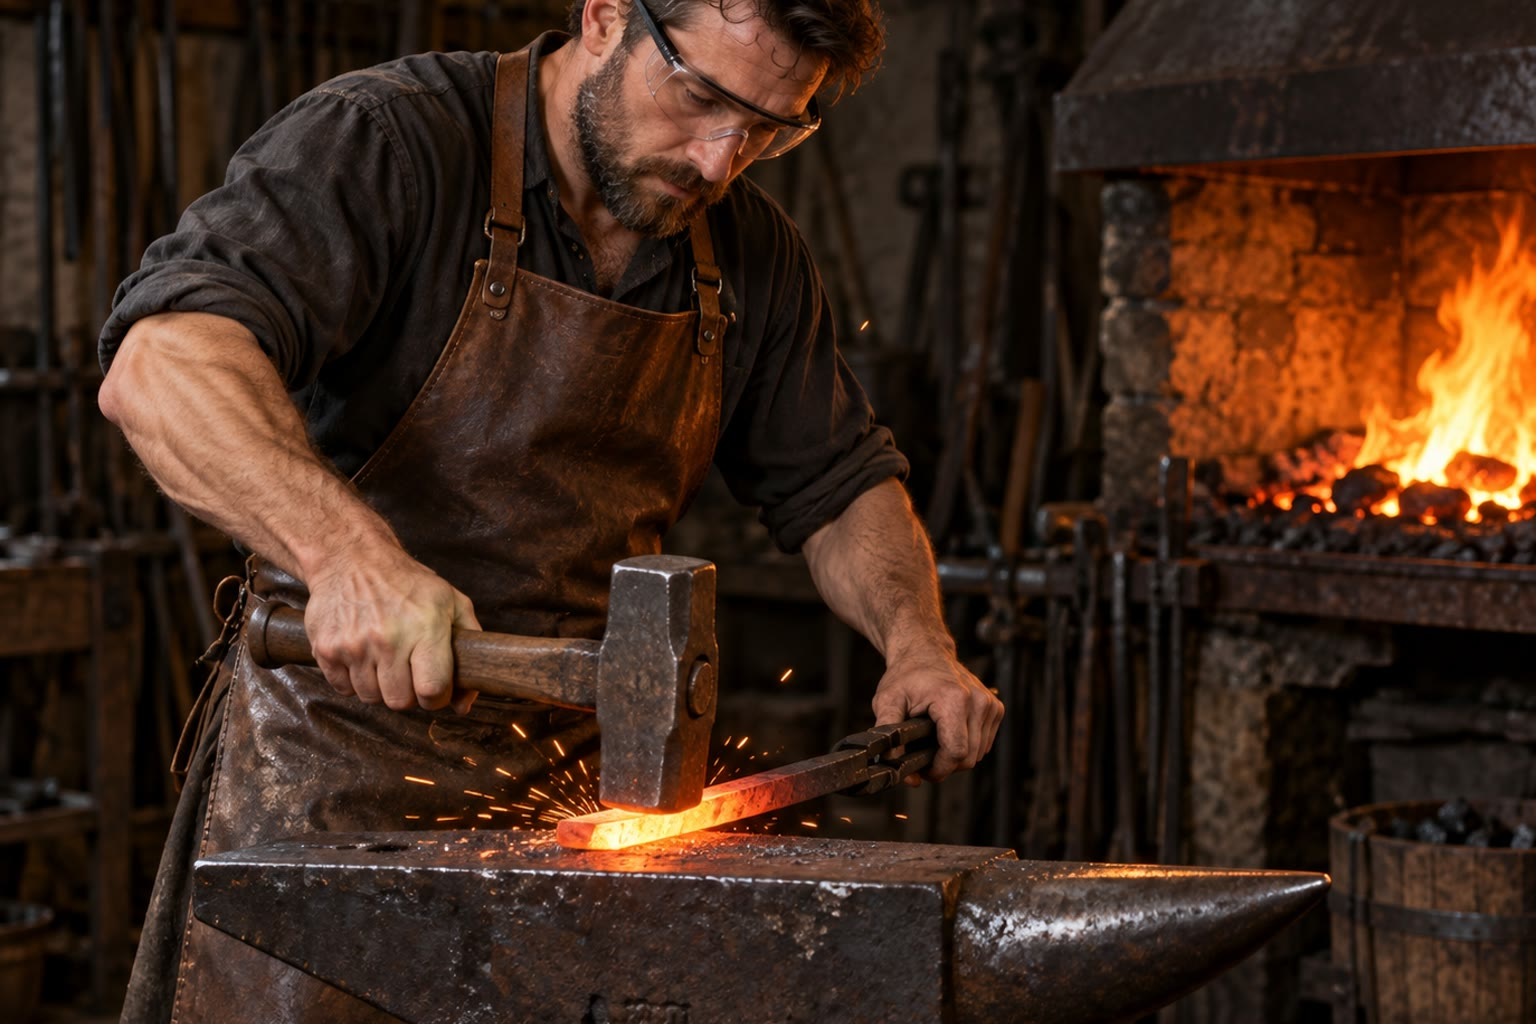
\includegraphics[width=0.55\linewidth]{images/book2/ai/b1-05-blacksmith.jpg}

{\small Un forgeron forgeant de l'acier. Le fer porté au rouge orangé a
une structure cristalline différente de celle du fer à température
ambiante, et peut contenir davantage de carbone (problème du week-end).}
\end{omfigure}

\section{Le modèle du cristal parfait}

\begin{definition}[Cristal, solide amorphe, cristal parfait]\label{def:b1:crystals-metals:crystal}
Un \emph{cristal}\index{cristal} est un solide dont les particules
(atomes, ions ou molécules) sont disposées selon un \omterm{def:b1:crystals-metals:lattice}{motif} qui se répète
périodiquement dans les trois dimensions. Un solide dépourvu de cet ordre
à longue distance est un \emph{solide amorphe}\index{solide amorphe}
(verre, la plupart des plastiques). Le \emph{modèle du cristal
parfait}\index{modele du cristal parfait@modèle du cristal parfait} décrit un cristal comme infini et sans défauts~:
ni atomes manquants ou en excès, ni impuretés, ni joints.
\end{definition}

\begin{definition}[Réseau, motif, maille]\label{def:b1:crystals-metals:lattice}
Un \emph{réseau}\index{reseau@réseau} est un ensemble infini de points, les
\emph{nœuds}\index{noeud@nœud}, obtenus à partir de l'un d'eux par toutes les
translations $u\,\vec a + v\,\vec b + w\,\vec c$ avec $u$, $v$, $w$
entiers. On obtient le \omterm{def:b1:crystals-metals:crystal}{cristal} en plaçant sur chaque nœud le même
\emph{motif}\index{motif} (un atome, un groupe d'atomes ou d'ions). Une
\emph{maille}\index{maille} est un parallélépipède construit sur
$\vec a$, $\vec b$, $\vec c$ dont les translations remplissent
l'espace~; les longueurs de ses arêtes et ses angles sont les
\emph{paramètres de maille}\index{parametres de maille@paramètres de maille}
$a$, $b$, $c$, $\alpha$, $\beta$, $\gamma$. Dans une maille cubique,
$a = b = c$ et les angles valent $90^\circ$.
\end{definition}

\begin{remark}[Cristaux réels]\label{rem:b1:crystals-metals:real}
Les \omterm{def:b1:crystals-metals:crystal}{cristaux} réels sont finis et imparfaits~: ils contiennent des
lacunes, des impuretés, des dislocations et des joints de grains, qui
gouvernent de nombreuses propriétés (la ductilité du cuivre, la dureté
de l'acier). Ces défauts sont étudiés dans le volume de troisième
année~; le \omterm{def:b1:crystals-metals:crystal}{cristal} parfait donne la géométrie, la masse volumique et la
\omterm{def:b1:crystals-metals:compactness}{compacité}, que les défauts modifient à peine.
\end{remark}

\begin{definition}[Multiplicité d'une maille]\label{def:b1:crystals-metals:multiplicity}
La \emph{multiplicité}\index{multiplicite@multiplicité} $Z$ d'une \omterm{def:b1:crystals-metals:lattice}{maille} (on dit aussi sa
population) est le nombre de \omterm{def:b1:crystals-metals:lattice}{motifs} (ou d'atomes) qui lui appartiennent,
chaque atome partagé avec les \omterm{def:b1:crystals-metals:lattice}{mailles} voisines comptant pour la fraction
qui se trouve à l'intérieur de la \omterm{def:b1:crystals-metals:lattice}{maille}.
\end{definition}

\begin{method}[Dénombrer les atomes d'une maille]\label{met:b1:crystals-metals:count}
Dans une \omterm{def:b1:crystals-metals:lattice}{maille} cubique, un atome situé à un sommet est partagé par 8
\omterm{def:b1:crystals-metals:lattice}{mailles} et compte pour $1/8$~; sur une arête, il est partagé par 4 et
compte pour $1/4$~; sur une face, il est partagé par 2 et compte pour
$1/2$~; à l'intérieur, il compte pour 1. Additionner les contributions.
\end{method}

\begin{definition}[Coordinence]\label{def:b1:crystals-metals:coordination}
La \emph{coordinence}\index{coordinence} d'une particule dans un solide
est le nombre de ses plus proches voisins, ceux qui se trouvent à la
plus courte distance.
\end{definition}

\begin{definition}[Compacité]\label{def:b1:crystals-metals:compactness}
La \emph{compacité}\index{compacite@compacité} (ou taux de remplissage) d'un
\omterm{def:b1:crystals-metals:crystal}{cristal} de sphères dures est la fraction du volume occupée par les
sphères~: pour une \omterm{def:b1:crystals-metals:lattice}{maille} de volume $V$ contenant $Z$ sphères de rayon
$R$,
\[
  C = \frac{Z \cdot \frac43 \pi R^3}{V} .
\]
\end{definition}

\begin{proposition}[Masse volumique à partir de la maille]\label{prop:b1:crystals-metals:density}
La masse volumique d'un \omterm{def:b1:crystals-metals:crystal}{cristal} dont la \omterm{def:b1:crystals-metals:lattice}{maille}, de volume $V$, contient
$Z$ particules de masse molaire $M$ vaut
\[
  \rho = \frac{Z\,M}{N_A\,V} .
\]
\end{proposition}

\begin{proof}
La \omterm{def:b1:crystals-metals:lattice}{maille} contient $Z$ particules, de masse $Z\,M/N_A$~; le \omterm{def:b1:crystals-metals:crystal}{cristal} est
la \omterm{def:b1:crystals-metals:lattice}{maille} répétée, sa masse volumique est donc celle d'une \omterm{def:b1:crystals-metals:lattice}{maille}.
\end{proof}

\section{Empilements compacts~: cubique à faces centrées et hexagonal}

\begin{definition}[Empilement compact, CFC, HC]\label{def:b1:crystals-metals:packings}
Un \emph{empilement compact}\index{empilement compact} de sphères identiques est formé de
couches compactes, dans lesquelles chaque sphère en touche six autres,
superposées de sorte que chaque sphère d'une couche repose dans un creux
de la couche inférieure. L'empilement $ABCABC\dots$ donne la structure
\emph{cubique à faces centrées}\index{cubique a faces centrees@cubique à faces centrées} (CFC)~; l'empilement $ABAB\dots$
donne la structure \emph{hexagonale compacte}\index{hexagonale compacte}
(HC). Une troisième structure des métaux, non compacte, est la structure
\emph{cubique centrée}\index{cubique centree@cubique centrée} (CC), un cube portant un atome à
chaque sommet et un en son centre.
\end{definition}

\begin{omfigure}
\begin{tikzpicture}[font=\small]
  % layer A
  \foreach \i in {0,...,4} \foreach \j in {0,...,3} {
    \pgfmathsetmacro\x{\i+0.5*\j}
    \pgfmathsetmacro\y{0.866*\j}
    \draw[black!60, fill=omDef!25] (\x,\y) circle (0.5);
  }
  % layer B, in the hollows pointing up
  \foreach \i/\j in {1/0, 2/0, 3/0, 1/1, 2/1, 3/1, 1/2, 2/2} {
    \pgfmathsetmacro\x{\i+0.5*\j}
    \pgfmathsetmacro\y{0.866*\j+0.577}
    \draw[omThm!80!black, fill=omThm!25, fill opacity=0.75] (\x,\y) circle (0.5);
  }
  % C positions
  \foreach \i/\j in {1/0, 2/0, 3/0, 1/1, 2/1, 3/1} {
    \pgfmathsetmacro\x{\i+0.5+0.5*\j}
    \pgfmathsetmacro\y{0.866*\j+0.289}
    \fill[omMeth] (\x,\y) circle (0.11);
  }
  \node[anchor=west, align=left] at (6.6,1.6) {A~: première couche (en bleu)\\B~: deuxième couche, dans\\\phantom{B~: }les creux de A (en rouge)\\C~: les autres creux\\\phantom{C~: }(points verts)};
\end{tikzpicture}

{\small Deux couches compactes vues de dessus. Une troisième couche peut
se placer au-dessus des creux marqués C (empilement $ABC$, \omterm{def:b1:crystals-metals:packings}{cubique à
faces centrées}) ou au-dessus des atomes de A (empilement $AB$,
hexagonal compact).}
\end{omfigure}

\begin{proposition}[Cubique à faces centrées]\label{prop:b1:crystals-metals:fcc}
Dans la structure CFC, les atomes occupent les huit sommets et les six
centres des faces d'un cube d'arête $a$. Alors $Z = 4$, la \omterm{def:b1:crystals-metals:coordination}{coordinence}
vaut 12, les atomes sont tangents le long d'une diagonale de face,
$a\sqrt2 = 4R$, et la \omterm{def:b1:crystals-metals:compactness}{compacité} vaut
\[
  C = \frac{\pi}{3\sqrt2} \approx 0.74 .
\]
\end{proposition}

\begin{proof}
$Z = 8 \times \frac18 + 6 \times \frac12 = 4$. Un atome au centre d'une
face touche les quatre sommets de sa face et les quatre centres de faces
de chacune des deux \omterm{def:b1:crystals-metals:lattice}{mailles} qui partagent cette face~: $4 + 4 + 4 = 12$
voisins à $a\sqrt2/2$. Sur une diagonale de face, de longueur $a\sqrt2$,
se trouvent un atome de sommet, un atome de centre de face et un atome
de sommet en contact~: $a\sqrt2 = 4R$. Alors
$C = 4 \cdot \frac43\pi R^3/a^3 = \frac{16}{3}\pi R^3/(2\sqrt2 R)^3 \cdot
\frac{1}{1} = \frac{16\pi}{3 \times 16\sqrt2} = \frac{\pi}{3\sqrt2}$.
\end{proof}

\begin{omfigure}
\tdplotsetmaincoords{60}{100}
\begin{tikzpicture}[tdplot_main_coords, font=\small]
  \pic {omcubeo={3}};
  \node[cellA=6mm] at (0,0,0) {};
  \node[cellA=6mm] at (0,3,0) {};
  \node[cellA=6mm, ball color=omDef!55] at (0,1.5,1.5) {};
  \node[cellA=6mm] at (0,0,3) {};
  \node[cellA=6mm, ball color=omDef!55] at (1.5,1.5,0) {};
  \node[cellA=6mm] at (0,3,3) {};
  \node[cellA=6mm, ball color=omDef!55] at (1.5,0,1.5) {};
  \node[cellA=6mm, ball color=omDef!55] at (1.5,3,1.5) {};
  \node[cellA=6mm] at (3,0,0) {};
  \node[cellA=6mm, ball color=omDef!55] at (1.5,1.5,3) {};
  \node[cellA=6mm] at (3,3,0) {};
  \node[cellA=6mm, ball color=omDef!55] at (3,1.5,1.5) {};
  \node[cellA=6mm] at (3,0,3) {};
  \node[cellA=6mm] at (3,3,3) {};
  \draw[omThm, thick] (3,0,0) -- (3,3,3);
\end{tikzpicture}
\hspace{1.2cm}
\begin{tikzpicture}[tdplot_main_coords, font=\small]
  \pic {omcubeo={3}};
  \node[cellA=7mm] at (0,0,0) {};
  \node[cellA=7mm] at (0,3,0) {};
  \node[cellA=7mm] at (0,0,3) {};
  \node[cellA=7mm] at (0,3,3) {};
  \node[cellA=7mm, ball color=omDef!55] at (1.5,1.5,1.5) {};
  \node[cellA=7mm] at (3,0,0) {};
  \node[cellA=7mm] at (3,3,0) {};
  \node[cellA=7mm] at (3,0,3) {};
  \node[cellA=7mm] at (3,3,3) {};
  \draw[omThm, thick] (3,0,0) -- (0,3,3);
\end{tikzpicture}

{\small À gauche~: la \omterm{def:b1:crystals-metals:lattice}{maille} \omterm{def:b1:crystals-metals:packings}{cubique à faces centrées} (atomes des
sommets en gris, atomes des centres des faces en bleu). Les atomes sont
tangents le long d'une diagonale de face (trait rouge, $a\sqrt2 = 4R$).
À droite~: la \omterm{def:b1:crystals-metals:lattice}{maille} \omterm{def:b1:crystals-metals:packings}{cubique centrée}~; les atomes sont tangents le long
de la grande diagonale (trait rouge, $a\sqrt3 = 4R$). Les atomes sont
dessinés plus petits que leur taille de contact, pour la clarté.}
\end{omfigure}

\begin{proposition}[Hexagonal compact]\label{prop:b1:crystals-metals:hcp}
Dans la structure HC, le prisme hexagonal conventionnel, d'arête de base
$a$ et de hauteur $c$, contient 6 atomes~; la \omterm{def:b1:crystals-metals:coordination}{coordinence} vaut 12~; pour
des sphères tangentes, $a = 2R$, $c/a = \sqrt{8/3} \approx 1.633$, et la
\omterm{def:b1:crystals-metals:compactness}{compacité} est la même que pour le CFC, $\pi/(3\sqrt2) \approx 0.74$.
\end{proposition}

\begin{proof}
Le prisme a 12 atomes aux sommets partagés par 6 prismes, 2 atomes aux
centres des faces partagés par 2, et 3 atomes intérieurs~:
$12/6 + 2/2 + 3 = 6$. Chaque atome touche six voisins dans sa couche et
trois dans chacune des couches adjacentes~: 12. Un atome de la couche B
repose sur trois atomes tangents de la couche A, avec lesquels il forme
un tétraèdre régulier d'arête $2R$, de hauteur $2R\sqrt{2/3}$~; deux
couches plus loin, $c = 4R\sqrt{2/3}$, donc $c/a = 2\sqrt{2/3} = \sqrt{8/3}$.
Le volume du prisme vaut $\frac{3\sqrt3}{2}a^2 c = \frac{3\sqrt3}{2}(2R)^2 \cdot
4R\sqrt{2/3} = 24\sqrt2\,R^3$, et $C = 6 \cdot \frac43\pi R^3/(24\sqrt2
R^3) = \pi/(3\sqrt2)$.
\end{proof}

\begin{omfigure}
\tdplotsetmaincoords{70}{113}
\begin{tikzpicture}[tdplot_main_coords, font=\small, scale=1.25]
  \pic[transform shape] {omhexprismo={1.6}{2.6}};
  \node[cellA=6mm] at (-1.6,0,0) {};
  \node[cellA=6mm] at (-0.8,-1.386,0) {};
  \node[cellA=6mm] at (-1.6,0,2.6) {};
  \node[cellA=6mm] at (-0.8,-1.386,2.6) {};
  \node[cellA=6mm] at (-0.8,1.386,0) {};
  \node[cellA=6mm, ball color=omThm!60] at (-0.8,0.462,1.3) {};
  \node[cellA=6mm] at (0,0,0) {};
  \node[cellA=6mm, ball color=omThm!60] at (0,-0.924,1.3) {};
  \node[cellA=6mm] at (0.8,-1.386,0) {};
  \node[cellA=6mm] at (-0.8,1.386,2.6) {};
  \node[cellA=6mm] at (0,0,2.6) {};
  \node[cellA=6mm] at (0.8,-1.386,2.6) {};
  \node[cellA=6mm] at (0.8,1.386,0) {};
  \node[cellA=6mm, ball color=omThm!60] at (0.8,0.462,1.3) {};
  \node[cellA=6mm] at (1.6,0,0) {};
  \node[cellA=6mm] at (0.8,1.386,2.6) {};
  \node[cellA=6mm] at (1.6,0,2.6) {};
\end{tikzpicture}

{\small Le prisme hexagonal compact, d'arête de base $a$ (le côté de
l'hexagone) et de hauteur $c$~: couches A (en gris) en bas et en haut,
couche B (en rouge) à mi-hauteur, logée dans les creux de A.}
\end{omfigure}

\section{Cubique centré et éléments métalliques}

\begin{proposition}[Cubique centré]\label{prop:b1:crystals-metals:bcc}
Dans la structure CC, $Z = 2$, la \omterm{def:b1:crystals-metals:coordination}{coordinence} vaut 8, les atomes sont
tangents le long de la grande diagonale du cube, $a\sqrt3 = 4R$, et la
\omterm{def:b1:crystals-metals:compactness}{compacité} vaut
\[
  C = \frac{\pi\sqrt3}{8} \approx 0.68 .
\]
\end{proposition}

\begin{proof}
$Z = 8 \times \frac18 + 1 = 2$. L'atome central touche les huit sommets~:
la grande diagonale $a\sqrt3$ porte un sommet, le centre et un sommet,
$a\sqrt3 = 4R$. Alors $C = 2 \cdot \frac43\pi R^3/a^3 =
\frac83\pi R^3 (\sqrt3/(4R))^3 = \frac83\pi \cdot \frac{3\sqrt3}{64} =
\frac{\pi\sqrt3}{8}$.
\end{proof}

\begin{proposition}[L'empilement compact est le plus dense]\label{prop:b1:crystals-metals:kepler}
Aucun empilement de sphères identiques n'a une \omterm{def:b1:crystals-metals:compactness}{compacité} supérieure à
$\pi/(3\sqrt2) \approx 0.7405$, la valeur du CFC et du HC.
\end{proposition}
\admitted

\begin{history}[La conjecture de Kepler, 1611--2017]
Dans un court essai sur les flocons de neige, écrit en 1611, Johannes
Kepler affirma qu'aucune façon d'empiler des boulets de canon ne pouvait
être plus dense que la pyramide de l'épicier, l'empilement \omterm{def:b1:crystals-metals:packings}{cubique à
faces centrées}. L'énoncé résista à toute démonstration pendant près de
quatre siècles. Thomas Hales en donna une preuve assistée par ordinateur
en 1998, et une preuve formelle vérifiée ligne à ligne par ordinateur
fut achevée en 2014 et publiée en 2017.
\end{history}

\begin{example}[Trois métaux]\label{ex:b1:crystals-metals:metals}
Le cuivre est CFC avec $a = \qty{361.5}{pm}$~: $R = a\sqrt2/4 =
\qty{127.8}{pm}$ et $\rho = 4 \times 63.55/(6.022 \times 10^{23} \times
(3.615 \times 10^{-8})^3) = \qty{8.93}{g/cm^3}$, la masse volumique
mesurée. Le fer à température ambiante (fer $\alpha$) est CC avec
$a = \qty{286.7}{pm}$~:
$R = \qty{124.1}{pm}$, $\rho = \qty{7.87}{g/cm^3}$. Le magnésium est HC
avec $a = \qty{320.9}{pm}$ et $c = \qty{521.0}{pm}$~: $c/a = 1.624$,
proche de la valeur idéale $1.633$~; le zinc, avec $c/a = 1.856$, est un
empilement hexagonal étiré.
% ledger: lat:Cu, rho:Cu, lat:Fe-alpha, rho:Fe, lat:Mg.a, lat:Mg.c,
% lat:Zn.a, lat:Zn.c, aw:Cu, aw:Fe, const:NA
\end{example}

\begin{center}
\small
\begin{tabular}{lllccc}
\hline
métal & structure & $a$ (pm) & $R$ (pm) & $\rho$ calculée & $\rho$ mesurée \\
\hline
aluminium & CFC & 405.0 & 143.2 & 2.70 & 2.70 \\
cuivre & CFC & 361.5 & 127.8 & 8.93 & 8.93 \\
argent & CFC & 408.6 & 144.5 & 10.50 & 10.50 \\
sodium & CC & 429.1 & 185.8 & 0.967 & 0.97 \\
fer $\alpha$ & CC & 286.7 & 124.1 & 7.87 & 7.87 \\
tungstène & CC & 316.5 & 137.0 & 19.26 & 19.3 \\
\hline
\end{tabular}
\end{center}
% ledger: lat:Al, lat:Cu, lat:Ag, lat:Na, lat:Fe-alpha, lat:W, rho:Al,
% rho:Cu, rho:Ag, rho:Na, rho:Fe, rho:W (densities in g/cm3)

\begin{omfigure}
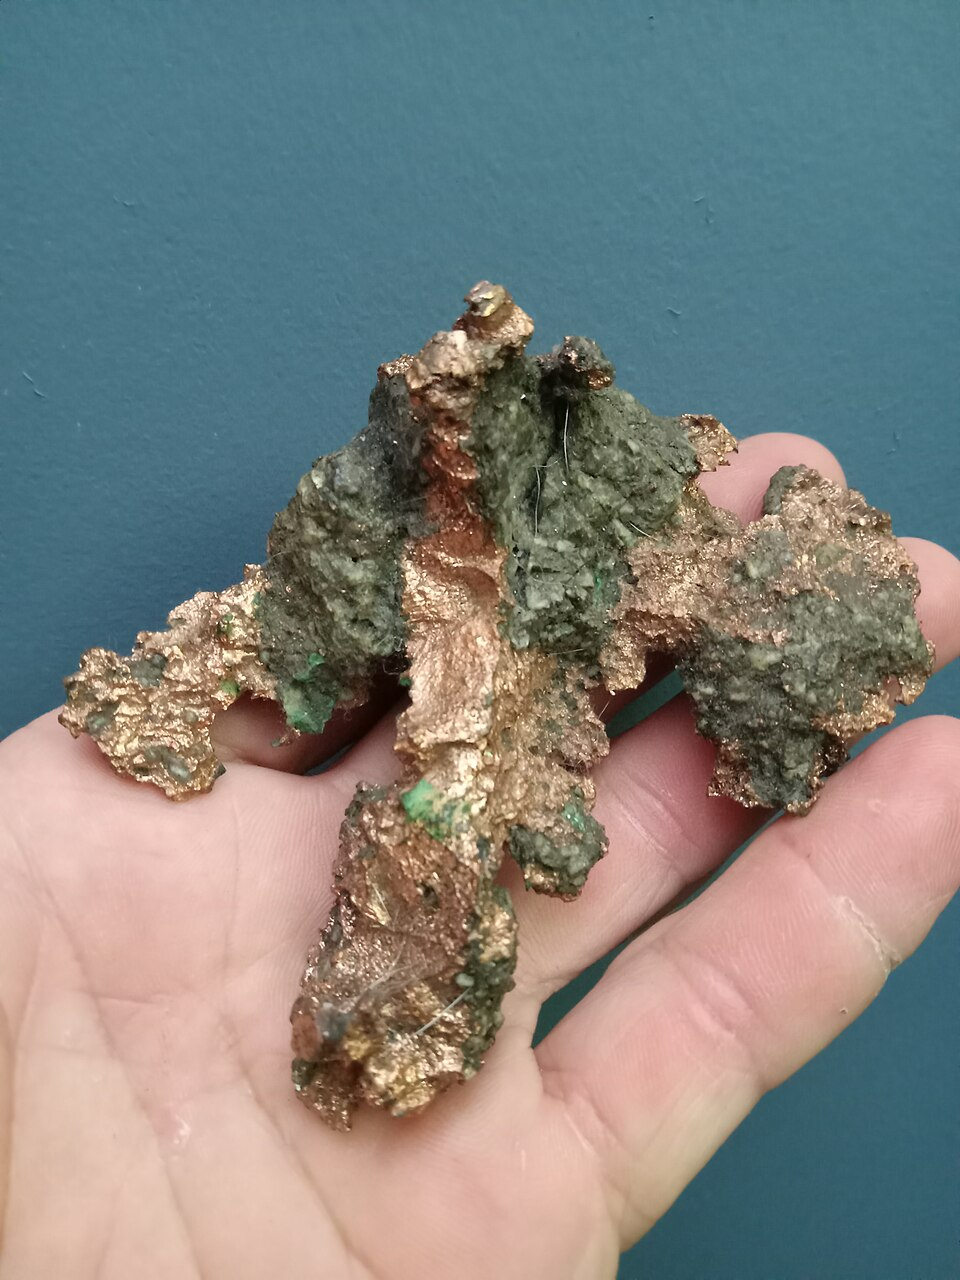
\includegraphics[width=0.36\linewidth]{images/book2/native-copper.jpg}

{\small Un échantillon de cuivre natif. Ses formes ramifiées ont poussé
comme des \omterm{def:b1:crystals-metals:crystal}{cristaux}~; le métal sous-jacent est une mosaïque de grains CFC.
Photo~: CC0 (Wikimedia Commons).}
\end{omfigure}

\section{Sites interstitiels}

\begin{definition}[Sites interstitiels]\label{def:b1:crystals-metals:site}
Un \emph{site interstitiel}\index{site interstitiel} est un espace vide entre les
atomes d'un \omterm{def:b1:crystals-metals:crystal}{cristal} où peut se loger un atome plus petit. Un \emph{site
tétraédrique}\index{site tetraedrique@site tétraédrique} se trouve au centre d'un tétraèdre de quatre
atomes, un \emph{site octaédrique}\index{site octaedrique@site octaédrique} au centre d'un
octaèdre de six. L'\emph{habitabilité}\index{habitabilite@habitabilité} d'un site est le rayon de
la plus grosse sphère qui peut s'y loger sans écarter les atomes qui
l'entourent.
\end{definition}

\begin{proposition}[Sites de la structure CFC]\label{prop:b1:crystals-metals:sites}
Une \omterm{def:b1:crystals-metals:lattice}{maille} CFC contient 4 \omterm{def:b1:crystals-metals:site}{sites octaédriques}, au centre du cube et aux
milieux de ses 12 arêtes, et 8 \omterm{def:b1:crystals-metals:site}{sites tétraédriques}, aux centres des 8
petits cubes d'arête $a/2$. Pour des atomes tangents de rayon $R$, les
\omterm{def:b1:crystals-metals:site}{habitabilités} valent
\[
  r_O = (\sqrt2 - 1)R \approx 0.414\,R, \qquad
  r_T = \left(\sqrt{\tfrac32} - 1\right)R \approx 0.225\,R .
\]
\end{proposition}

\begin{proof}
\omterm{def:b1:crystals-metals:site}{Sites octaédriques}~: $1 + 12 \times \frac14 = 4$, autant que d'atomes.
Le centre du cube est à $a/2$ des six centres des faces~: $r_O + R = a/2$
avec $a = 2\sqrt2 R$, donc $r_O = (\sqrt2 - 1)R$. \omterm{def:b1:crystals-metals:site}{Sites tétraédriques}~:
le centre d'un petit cube d'arête $a/2$ est à une demi-grande diagonale,
$\frac{a}{2}\cdot\frac{\sqrt3}{2} = \frac{a\sqrt3}{4}$, des quatre atomes
situés à des sommets alternés~: $r_T + R = \frac{\sqrt3}{4}\,2\sqrt2\,R =
\sqrt{\tfrac32}\,R$.
\end{proof}

\begin{omfigure}
\tdplotsetmaincoords{60}{100}
\begin{tikzpicture}[tdplot_main_coords, font=\small]
  \pic {omcubeo={3}};
  \node[cellA=3.6mm] at (0,0,0) {};
  \node[cellsite=4mm, draw=omThm, fill=omThm!30] at (0,1.5,0) {};
  \node[cellA=3.6mm] at (0,3,0) {};
  \node[cellsite=4mm, draw=omThm, fill=omThm!30] at (0,0,1.5) {};
  \node[cellA=3.6mm] at (0,1.5,1.5) {};
  \node[cellsite=4mm, draw=omThm, fill=omThm!30] at (0,3,1.5) {};
  \node[cellsite=4mm, draw=omThm, fill=omThm!30] at (1.5,0,0) {};
  \node[cellA=3.6mm] at (0,0,3) {};
  \node[cellA=3.6mm] at (1.5,1.5,0) {};
  \node[cellsite=4mm, draw=omThm, fill=omThm!30] at (0,1.5,3) {};
  \node[cellsite=4mm, draw=omThm, fill=omThm!30] at (1.5,3,0) {};
  \node[cellA=3.6mm] at (0,3,3) {};
  \node[cellA=3.6mm] at (1.5,0,1.5) {};
  \node[cellsite=5mm, draw=omThm, fill=omThm!30] at (1.5,1.5,1.5) {};
  \node[cellA=3.6mm] at (1.5,3,1.5) {};
  \node[cellA=3.6mm] at (3,0,0) {};
  \node[cellsite=4mm, draw=omThm, fill=omThm!30] at (1.5,0,3) {};
  \node[cellsite=4mm, draw=omThm, fill=omThm!30] at (3,1.5,0) {};
  \node[cellA=3.6mm] at (1.5,1.5,3) {};
  \node[cellA=3.6mm] at (3,3,0) {};
  \node[cellsite=4mm, draw=omThm, fill=omThm!30] at (1.5,3,3) {};
  \node[cellsite=4mm, draw=omThm, fill=omThm!30] at (3,0,1.5) {};
  \node[cellA=3.6mm] at (3,1.5,1.5) {};
  \node[cellsite=4mm, draw=omThm, fill=omThm!30] at (3,3,1.5) {};
  \node[cellA=3.6mm] at (3,0,3) {};
  \node[cellsite=4mm, draw=omThm, fill=omThm!30] at (3,1.5,3) {};
  \node[cellA=3.6mm] at (3,3,3) {};
  \node[below] at (1.5,1.5,-1.5) {sites octaédriques (en rouge)};
\end{tikzpicture}
\hspace{1.2cm}
\begin{tikzpicture}[tdplot_main_coords, font=\small]
  \pic {omcubeo={3}};
  \node[cellA=3.6mm] at (0,0,0) {};
  \node[cellA=3.6mm] at (0,3,0) {};
  \node[cellA=3.6mm] at (0,1.5,1.5) {};
  \node[cellsite=4mm, fill=omDef!30] at (0.75,0.75,0.75) {};
  \node[cellsite=4mm, fill=omDef!30] at (0.75,2.25,0.75) {};
  \node[cellA=3.6mm] at (0,0,3) {};
  \node[cellA=3.6mm] at (1.5,1.5,0) {};
  \node[cellsite=4mm, fill=omDef!30] at (0.75,0.75,2.25) {};
  \node[cellA=3.6mm] at (0,3,3) {};
  \node[cellA=3.6mm] at (1.5,0,1.5) {};
  \node[cellsite=4mm, fill=omDef!30] at (0.75,2.25,2.25) {};
  \node[cellsite=4mm, fill=omDef!30] at (2.25,0.75,0.75) {};
  \node[cellA=3.6mm] at (1.5,3,1.5) {};
  \node[cellA=3.6mm] at (3,0,0) {};
  \node[cellsite=4mm, fill=omDef!30] at (2.25,2.25,0.75) {};
  \node[cellA=3.6mm] at (1.5,1.5,3) {};
  \node[cellA=3.6mm] at (3,3,0) {};
  \node[cellsite=4mm, fill=omDef!30] at (2.25,0.75,2.25) {};
  \node[cellsite=4mm, fill=omDef!30] at (2.25,2.25,2.25) {};
  \node[cellA=3.6mm] at (3,1.5,1.5) {};
  \node[cellA=3.6mm] at (3,0,3) {};
  \node[cellA=3.6mm] at (3,3,3) {};
  \draw[omDef!70!black, thin] (0,0,0) -- (0.75,0.75,0.75) -- (1.5,1.5,0)
    (0.75,0.75,0.75) -- (1.5,0,1.5) (0.75,0.75,0.75) -- (0,1.5,1.5);
  \node[below] at (1.5,1.5,-1.5) {sites tétraédriques (en bleu)};
\end{tikzpicture}

{\small \omterm{def:b1:crystals-metals:site}{Sites interstitiels} de la \omterm{def:b1:crystals-metals:lattice}{maille} CFC. À gauche~: le \omterm{def:b1:crystals-metals:site}{site
octaédrique} au centre et ceux des milieux des arêtes (partagés par
quatre \omterm{def:b1:crystals-metals:lattice}{mailles}). À droite~: les huit \omterm{def:b1:crystals-metals:site}{sites tétraédriques} aux centres des
huitièmes du cube, l'un d'eux relié à ses quatre atomes.}
\end{omfigure}

\section{Liaison métallique et alliages}

\begin{definition}[Liaison métallique]\label{def:b1:crystals-metals:metallic-bond}
Dans la \emph{liaison métallique}\index{liaison metallique@liaison métallique}, chaque atome d'un
métal cède ses \omterm{def:b1:quantum-numbers:configuration}{électrons de valence} à l'ensemble du \omterm{def:b1:crystals-metals:crystal}{cristal}~: le solide
est un \omterm{def:b1:crystals-metals:lattice}{réseau} de cations baignant dans des électrons qui n'appartiennent
à aucun atome en particulier et s'y déplacent librement. La liaison est
l'attraction entre les cations et ce nuage d'électrons partagé~; elle
n'est pas dirigée.
\end{definition}

\begin{proposition}[Propriétés des métaux]\label{prop:b1:crystals-metals:properties}
La \omterm{def:b1:crystals-metals:metallic-bond}{liaison métallique} explique les propriétés des métaux~: les électrons
mobiles conduisent l'électricité et la chaleur et réfléchissent la
lumière (éclat)~; comme la liaison n'est pas dirigée, des plans d'atomes
peuvent glisser les uns sur les autres sans briser le \omterm{def:b1:crystals-metals:crystal}{cristal}
(ductilité, malléabilité), et les \omterm{def:b1:crystals-metals:packings}{empilements compacts}, qui maximisent
le nombre de voisins, sont les structures les plus courantes.
\end{proposition}
\admitted

\begin{definition}[Alliages]\label{def:b1:crystals-metals:alloy}
Un alliage est un solide métallique formé de plusieurs éléments. Dans un
\emph{alliage de substitution}\index{alliage de substitution}, les atomes
de l'élément ajouté remplacent des atomes de l'hôte sur son \omterm{def:b1:crystals-metals:lattice}{réseau}~; il
faut pour cela des rayons qui ne diffèrent pas de plus de 15\,\% environ
(cuivre et nickel, cuivre et zinc dans le laiton). Dans un
\emph{alliage d'insertion}\index{alliage d'insertion}, de petits atomes
(\ce{H}, \ce{C}, \ce{N}, \ce{B}) occupent des \omterm{def:b1:crystals-metals:site}{sites interstitiels} de
l'hôte (le carbone dans l'acier).
\end{definition}

\begin{definition}[Allotropie]\label{def:b1:crystals-metals:allotropy}
Les différentes structures cristallines d'un même élément sont ses
\emph{variétés allotropiques}\index{variete allotropique@variété allotropique}. Le fer est CC (fer $\alpha$) à
température ambiante~; on l'a mesuré CFC (fer $\gamma$) de
\qty{1189}{K} à \qty{1661}{K}, puis de nouveau CC (fer $\delta$) à
\qty{1662}{K}, jusqu'à sa fusion. Le carbone existe sous forme de
diamant et de graphite (\cref{ch:b1:crystals-ionic-covalent}).
% ledger: lat:Fe-alpha, lat:Fe-gamma-1189, lat:Fe-gamma-1661,
% lat:Fe-delta-1662
\end{definition}

\begin{example}[L'acier]\label{ex:b1:crystals-metals:steel}
Le carbone, de \omterm{def:b1:periodicity:radius}{rayon covalent} \qty{77}{pm} (la moitié de la distance
\ce{C-C} dans le diamant), est trop gros pour les sites du fer sans les
déformer, mais beaucoup moins dans le fer $\gamma$, dont les \omterm{def:b1:crystals-metals:site}{sites
octaédriques} sont les plus grands. On fabrique l'acier en dissolvant du
carbone dans du fer $\gamma$ chaud~; par trempe, le carbone reste piégé
quand le fer revient à une structure \omterm{def:b1:crystals-metals:packings}{cubique centrée}, qu'il déforme, et
le \omterm{def:b1:crystals-metals:crystal}{cristal} déformé est dur.
% ledger: lat:C-diamond (r = a sqrt3 / 8 = 77.2 pm)
\end{example}

\begin{remark}[Les transitions du fer]\label{rem:b1:crystals-metals:iron-T}
Les températures de la \cref{def:b1:crystals-metals:allotropy} sont
celles du fer pur à la pression atmosphérique~; le carbone dissous
abaisse la température à laquelle se forme le fer $\gamma$, ce qui rend
l'acier facile à travailler. Les diagrammes de phases des alliages sont
étudiés dans le volume de deuxième année.
\end{remark}

\section{Exercices}

\begin{exercise}[$\star$]\label{exo:b1:crystals-metals:1}
Dénombrer les atomes d'une \omterm{def:b1:crystals-metals:lattice}{maille} cubique simple (atomes aux sommets
seulement), d'une \omterm{def:b1:crystals-metals:lattice}{maille} CC et d'une \omterm{def:b1:crystals-metals:lattice}{maille} CFC, et donner la \omterm{def:b1:crystals-metals:coordination}{coordinence}
dans chaque cas.
\end{exercise}

\begin{exercise}[$\star$]\label{exo:b1:crystals-metals:2}
Montrer que la \omterm{def:b1:crystals-metals:compactness}{compacité} de la structure cubique simple (atomes tangents
le long d'une arête) vaut $\pi/6$, et comparer avec le CFC et le CC.
\end{exercise}

\begin{exercise}[$\star$]\label{exo:b1:crystals-metals:3}
L'aluminium est CFC avec $a = \qty{405.0}{pm}$. Calculer son rayon
atomique et sa masse volumique ($M = \qty{26.98}{g/mol}$).
% ledger: lat:Al, aw:Al
\end{exercise}

\begin{exercise}[$\star$]\label{exo:b1:crystals-metals:4}
Le sodium est CC avec $a = \qty{429.1}{pm}$. Calculer son rayon atomique
et sa masse volumique ($M = \qty{22.99}{g/mol}$), et comparer à la valeur
mesurée, \qty{0.97}{g/cm^3}.
% ledger: lat:Na, rho:Na, aw:Na
\end{exercise}

\begin{exercise}[$\star\star$]\label{exo:b1:crystals-metals:5}
L'argent est CFC et sa masse volumique vaut \qty{10.50}{g/cm^3}
($M = \qty{107.87}{g/mol}$). Calculer le paramètre de \omterm{def:b1:crystals-metals:lattice}{maille} et le rayon
atomique.
% ledger: rho:Ag, aw:Ag
\end{exercise}

\begin{exercise}[$\star\star$]\label{exo:b1:crystals-metals:6}
Montrer que, dans une structure HC de sphères tangentes,
$c/a = \sqrt{8/3}$. Le magnésium a $a = \qty{320.9}{pm}$,
$c = \qty{521.0}{pm}$. Calculer $c/a$ et la masse volumique du
magnésium ($M = \qty{24.31}{g/mol}$).
% ledger: lat:Mg.a, lat:Mg.c, aw:Mg
\end{exercise}

\begin{exercise}[$\star\star$]\label{exo:b1:crystals-metals:7}
Dans une \omterm{def:b1:crystals-metals:lattice}{maille} CFC d'arête $a$, donner les coordonnées des 4 atomes qui
appartiennent à la \omterm{def:b1:crystals-metals:lattice}{maille}, des 4 \omterm{def:b1:crystals-metals:site}{sites octaédriques} et des 8 \omterm{def:b1:crystals-metals:site}{sites
tétraédriques}. Combien de chaque par atome~?
\end{exercise}

\begin{exercise}[$\star\star$]\label{exo:b1:crystals-metals:8}
Le cuivre et le nickel sont tous deux CFC, avec $a = \qty{361.5}{pm}$ et
$a = \qty{352.4}{pm}$. Calculer leurs rayons atomiques. Ils forment un
\omterm{def:b1:crystals-metals:alloy}{alliage de substitution} en toutes proportions~: expliquer. Quel type
d'alliage l'hydrogène, atome très petit, peut-il former avec un métal~?
% ledger: lat:Cu, lat:Ni
\end{exercise}

\begin{exercise}[$\star\star$]\label{exo:b1:crystals-metals:9}
Le tungstène est CC avec $a = \qty{316.5}{pm}$. Calculer son rayon, sa
masse volumique ($M = \qty{183.84}{g/mol}$) et le nombre d'atomes dans
\qty{1}{cm^3}.
% ledger: lat:W, aw:W
\end{exercise}

\begin{exercise}[$\star\star\star$]\label{exo:b1:crystals-metals:10}
Dans la structure CC, un \omterm{def:b1:crystals-metals:site}{site octaédrique} se trouve au centre de chaque
face (et au milieu de chaque arête), et un \omterm{def:b1:crystals-metals:site}{site tétraédrique} en
$(\frac{a}{2}, \frac{a}{4}, 0)$ sur chaque face. Montrer que leurs
\omterm{def:b1:crystals-metals:site}{habitabilités} valent $r_O = \frac{2 - \sqrt3}{4}\,a$ et
$r_T = \frac{\sqrt5 - \sqrt3}{4}\,a$, et les exprimer en fractions de
$R$. Quel site est le plus grand~?
\end{exercise}

\begin{exercise}[$\star\star\star$]\label{exo:b1:crystals-metals:11}
Un métal cristallise avec $Z$ atomes par \omterm{def:b1:crystals-metals:lattice}{maille} cubique d'arête $a$.
Montrer que la \omterm{def:b1:crystals-metals:compactness}{compacité} peut s'écrire $C = \frac{4\pi R^3 Z}{3a^3}$,
puis que
$C = \frac{\pi\rho N_A}{6M}\,(2R)^3$. Appliquer au cuivre ($R = \qty{127.8}{pm}$,
$\rho = \qty{8.93}{g/cm^3}$) pour vérifier la valeur $0.74$.
\end{exercise}

\begin{exercise}[$\star\star\star$]\label{exo:b1:crystals-metals:12}
L'or est CFC avec $a = \qty{407.8}{pm}$ et l'argent CFC avec
$a = \qty{408.6}{pm}$. L'or et l'argent se mélangent en toutes
proportions. Estimer le paramètre de \omterm{def:b1:crystals-metals:lattice}{maille} d'un alliage à 50\,\%
d'atomes de chacun (prendre la moyenne) et sa masse volumique
($M(\ce{Au}) = \qty{196.97}{g/mol}$,
$M(\ce{Ag}) = \qty{107.87}{g/mol}$).
% ledger: lat:Au, lat:Ag, aw:Au, aw:Ag
\end{exercise}

\section{Problème~: pourquoi l'acier retient le carbone}

\begin{problem}[{Problème du week-end --- le fer au-dessous et au-dessus
de sa transition vers 1190\,K, les vides entre ses atomes, et la place
qu'ils laissent au carbone}]
\label{pb:b1:crystals-metals:1}
Données~: $M(\ce{Fe}) = \qty{55.845}{g/mol}$, $M(\ce{C}) = \qty{12.011}{g/mol}$,
$N_A = \qty{6.022e23}{mol^{-1}}$. À température ambiante, le fer
$\alpha$ est CC avec $a = \qty{286.65}{pm}$. À \qty{1189}{K}, juste
au-dessus de la transition, on mesure pour le fer $\alpha$ (encore
présent sous la transition) $a = \qty{289.8}{pm}$ et pour le fer
$\gamma$, CFC, $a = \qty{363.9}{pm}$. Le diamant est cubique avec
$a = \qty{356.68}{pm}$, chaque carbone en touchant quatre autres au
quart de la grande diagonale.
% ledger: lat:Fe-alpha, lat:Fe-alpha-1189, lat:Fe-gamma-1189,
% lat:C-diamond, aw:Fe, aw:C, const:NA

\medskip
\noindent\textbf{Partie I --- Le fer $\alpha$ à température ambiante.}
\begin{enumerate}
  \item Combien d'atomes appartiennent à une \omterm{def:b1:crystals-metals:lattice}{maille} CC~? Quelle est la
        \omterm{def:b1:crystals-metals:coordination}{coordinence}~?
  \item Le long de quelle ligne les atomes sont-ils tangents~? Calculer
        le rayon d'un atome de fer.
  \item Calculer la masse volumique du fer $\alpha$.
  \item Combien d'atomes de fer \qty{1}{cm^3} de fer $\alpha$
        contient-il~?
  \item Calculer la \omterm{def:b1:crystals-metals:compactness}{compacité} de la structure CC.
  \item Comparer à la masse volumique mesurée, \qty{7.87}{g/cm^3}.
% ledger: rho:Fe
\end{enumerate}

\medskip
\noindent\textbf{Partie II --- Franchir la transition.}
\begin{enumerate}[resume]
  \item Calculer le rayon d'un atome de fer dans le fer $\alpha$ et dans
        le fer $\gamma$ à \qty{1189}{K}.
  \item Calculer le volume par atome dans chaque phase.
  \item Quelle phase est la plus dense~? Calculer les deux masses
        volumiques.
  \item De quel pourcentage le volume d'une barre varie-t-il quand elle
        passe de $\alpha$ à $\gamma$ au chauffage~?
  \item Le résultat est-il cohérent avec les \omterm{def:b1:crystals-metals:compactness}{compacités} des deux
        structures~?
\end{enumerate}

\medskip
\noindent\textbf{Partie III --- Les vides du fer $\alpha$.}
\begin{enumerate}[resume]
  \item À partir de la structure du diamant, calculer le \omterm{def:b1:periodicity:radius}{rayon covalent}
        du carbone.
  \item Dans le fer $\alpha$ CC à \qty{1189}{K}, calculer l'\omterm{def:b1:crystals-metals:site}{habitabilité}
        d'un \omterm{def:b1:crystals-metals:site}{site octaédrique}, $r_O = \frac{2 - \sqrt3}{4}\,a$.
  \item Calculer celle d'un \omterm{def:b1:crystals-metals:site}{site tétraédrique}, $r_T = \frac{\sqrt5 -
        \sqrt3}{4}\,a$.
  \item Comparer au rayon du carbone. Que doit-il arriver au \omterm{def:b1:crystals-metals:lattice}{réseau}
        autour d'un atome de carbone~?
  \item Expliquer pourquoi le carbone ne se dissout qu'en quantités
        infimes dans le fer $\alpha$.
\end{enumerate}

\medskip
\noindent\textbf{Partie IV --- Les vides du fer $\gamma$.}
\begin{enumerate}[resume]
  \item Combien de \omterm{def:b1:crystals-metals:site}{sites octaédriques} une \omterm{def:b1:crystals-metals:lattice}{maille} CFC de fer $\gamma$
        contient-elle, par atome de fer~?
  \item Calculer l'\omterm{def:b1:crystals-metals:site}{habitabilité} d'un \omterm{def:b1:crystals-metals:site}{site tétraédrique} du fer $\gamma$.
  \item Si tous les \omterm{def:b1:crystals-metals:site}{sites octaédriques} étaient occupés par du carbone,
        quelle serait la formule du solide et la fraction massique en
        carbone~?
  \item Si un \omterm{def:b1:crystals-metals:site}{site octaédrique} sur dix était occupé, que vaudrait la
        fraction massique en carbone~?
  \item Expliquer pourquoi l'on fabrique l'acier en dissolvant du
        carbone dans du fer chaud.
  \item Calculer le rayon de la plus grosse sphère qui peut se loger
        dans un \omterm{def:b1:crystals-metals:site}{site octaédrique} du fer $\gamma$.
\end{enumerate}
\end{problem}
